% Options for packages loaded elsewhere
\PassOptionsToPackage{unicode}{hyperref}
\PassOptionsToPackage{hyphens}{url}
%
\documentclass[
]{book}
\usepackage{amsmath,amssymb}
\usepackage{lmodern}
\usepackage{ifxetex,ifluatex}
\ifnum 0\ifxetex 1\fi\ifluatex 1\fi=0 % if pdftex
  \usepackage[T1]{fontenc}
  \usepackage[utf8]{inputenc}
  \usepackage{textcomp} % provide euro and other symbols
\else % if luatex or xetex
  \usepackage{unicode-math}
  \defaultfontfeatures{Scale=MatchLowercase}
  \defaultfontfeatures[\rmfamily]{Ligatures=TeX,Scale=1}
\fi
% Use upquote if available, for straight quotes in verbatim environments
\IfFileExists{upquote.sty}{\usepackage{upquote}}{}
\IfFileExists{microtype.sty}{% use microtype if available
  \usepackage[]{microtype}
  \UseMicrotypeSet[protrusion]{basicmath} % disable protrusion for tt fonts
}{}
\makeatletter
\@ifundefined{KOMAClassName}{% if non-KOMA class
  \IfFileExists{parskip.sty}{%
    \usepackage{parskip}
  }{% else
    \setlength{\parindent}{0pt}
    \setlength{\parskip}{6pt plus 2pt minus 1pt}}
}{% if KOMA class
  \KOMAoptions{parskip=half}}
\makeatother
\usepackage{xcolor}
\IfFileExists{xurl.sty}{\usepackage{xurl}}{} % add URL line breaks if available
\IfFileExists{bookmark.sty}{\usepackage{bookmark}}{\usepackage{hyperref}}
\hypersetup{
  pdftitle={偏微分方程},
  pdfauthor={谭皓文},
  hidelinks,
  pdfcreator={LaTeX via pandoc}}
\urlstyle{same} % disable monospaced font for URLs
\usepackage{longtable,booktabs,array}
\usepackage{calc} % for calculating minipage widths
% Correct order of tables after \paragraph or \subparagraph
\usepackage{etoolbox}
\makeatletter
\patchcmd\longtable{\par}{\if@noskipsec\mbox{}\fi\par}{}{}
\makeatother
% Allow footnotes in longtable head/foot
\IfFileExists{footnotehyper.sty}{\usepackage{footnotehyper}}{\usepackage{footnote}}
\makesavenoteenv{longtable}
\usepackage{graphicx}
\makeatletter
\def\maxwidth{\ifdim\Gin@nat@width>\linewidth\linewidth\else\Gin@nat@width\fi}
\def\maxheight{\ifdim\Gin@nat@height>\textheight\textheight\else\Gin@nat@height\fi}
\makeatother
% Scale images if necessary, so that they will not overflow the page
% margins by default, and it is still possible to overwrite the defaults
% using explicit options in \includegraphics[width, height, ...]{}
\setkeys{Gin}{width=\maxwidth,height=\maxheight,keepaspectratio}
% Set default figure placement to htbp
\makeatletter
\def\fps@figure{htbp}
\makeatother
\setlength{\emergencystretch}{3em} % prevent overfull lines
\providecommand{\tightlist}{%
  \setlength{\itemsep}{0pt}\setlength{\parskip}{0pt}}
\setcounter{secnumdepth}{5}
\usepackage{ctex}

%\usepackage{xltxtra} % XeLaTeX的一些额外符号
% 设置中文字体
%\setCJKmainfont[BoldFont={黑体},ItalicFont={楷体}]{新宋体}

% 设置边距
\usepackage{geometry}
\geometry{%
  left=2.0cm, right=2.0cm, top=3.5cm, bottom=2.5cm} 

\usepackage{amsthm,mathrsfs}
\usepackage{booktabs}
\usepackage{longtable}
\makeatletter
\def\thm@space@setup{%
  \thm@preskip=8pt plus 2pt minus 4pt
  \thm@postskip=\thm@preskip
}
\makeatother
\ifluatex
  \usepackage{selnolig}  % disable illegal ligatures
\fi
\usepackage[style=apa,]{biblatex}
\addbibresource{mybib.bib}

\title{偏微分方程}
\author{谭皓文}
\date{2021年9月1日}

\begin{document}
\maketitle

{
\setcounter{tocdepth}{1}
\tableofcontents
}
\hypertarget{ux5bfcux8a00}{%
\chapter*{导言}\label{ux5bfcux8a00}}
\addcontentsline{toc}{chapter}{导言}

偏微分方程又叫数学物理方程,是在常微分方程的基础上的更难的一门学科,其中我们会遇到许多不同的问题,和之前的常微分相比,特点为方法并不通用,并且要求一定的物理知识,如果不同的问题使用错误的方法是做不出来的。因此我们需要大量的练习。

参考书:

\begin{itemize}
\tightlist
\item
  姜礼尚《数学物理方程》
\item
  周蜀林《偏微分方程》
\end{itemize}

学习内容是前五章

\hypertarget{ux6ce2ux52a8ux65b9ux7a0b}{%
\chapter{波动方程}\label{ux6ce2ux52a8ux65b9ux7a0b}}

\hypertarget{ux5f26ux632fux52a8ux65b9ux7a0b}{%
\section{弦振动方程}\label{ux5f26ux632fux52a8ux65b9ux7a0b}}

\hypertarget{ux65b9ux7a0bux7684ux5bfcux51faux5b9aux89e3ux6761ux4ef6}{%
\subsection{方程的导出、定解条件}\label{ux65b9ux7a0bux7684ux5bfcux51faux5b9aux89e3ux6761ux4ef6}}

\hypertarget{ux5f26ux632fux52a8ux65b9ux7a0b-1}{%
\subsubsection{弦振动方程}\label{ux5f26ux632fux52a8ux65b9ux7a0b-1}}

\(u(x,t)\)表示每点\(x\)在时刻\(t\)的位移。

其中我们需要做出以下假设以简化问题,因此我们做出如下假设,也叫理想假设(没有外力):

\begin{enumerate}
\def\labelenumi{\arabic{enumi}.}
\tightlist
\item
  弦是均匀的,换言之则是线密度为常数,并且,直径//长度\textless\textless1,也就是说,直径比长度远小。这个保证弦可以看作是理想中的一条线。
\item
  弦在某一平面是做微小的横振动(运动方向与传播方向垂直)。这个保证了弦没有发生巨大形变。
\item
  弦是柔软的,并且张力方向与切线方向一致。也就是说满足胡克定律,张力的大小与形变大小成正比。
\end{enumerate}

我们需要了解的知识点

\begin{itemize}
\tightlist
\item
  牛顿第二定律:\(F=ma,Ft=mv\)
\item
  在\((x,x + \Delta x)\)上,弧长\(S = \int_{x}^{x+\Delta x} \sqrt{1+(\frac{\partial u}{\partial x})^2} dx \approx \int_{x}^{x+\Delta x} dx = \Delta x\)
\end{itemize}

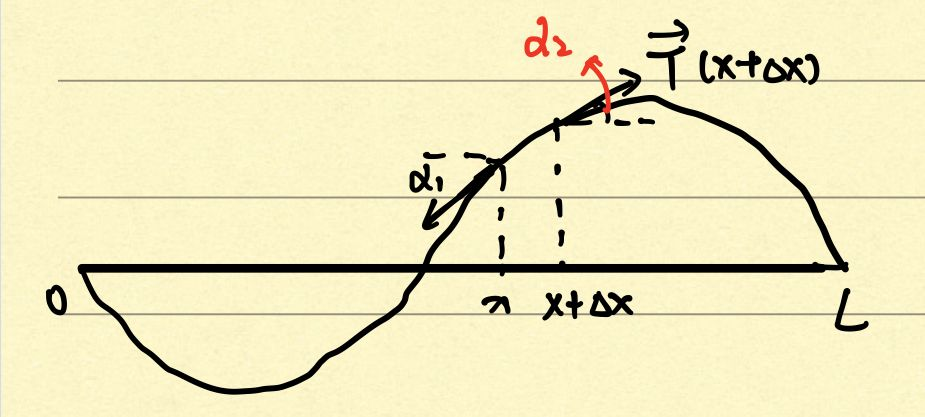
\includegraphics{t1.jpg}
在如上的力学分析示图中我们可以设在\(x\)点处的张力\(\vec{T}(x)=\),并且\(T(x)= \lvert\vec{T}(x) \lvert\)。

\begin{longtable}[]{@{}lll@{}}
\toprule
& 水平分力 & 竖直分力 \\
\midrule
\endhead
\(x\) & \(-T(x)cos\alpha_1\) & \(-T(x)sin\alpha_1\) \\
\(x+\Delta x\) & \(T(x+\Delta x)cos\alpha_2\) & \(T(x+\Delta x)sin\alpha_2\) \\
\bottomrule
\end{longtable}

\hypertarget{causal}{%
\chapter{格兰格因果性}\label{causal}}

\printbibliography

\end{document}
